\documentclass[a4paper,10pt]{article}
\usepackage[spanish]{babel}
\usepackage[utf8]{inputenc}
\usepackage{hyperref}
\usepackage{multicol}
\usepackage{geometry}
\usepackage{graphicx}
\usepackage{wrapfig}
\usepackage{subcaption}
\usepackage{lipsum}
\newcommand*{\airbnb}{\textit{Airbnb}}
\newcommand*{\webscrapping}{\textit{web scrapping}}

\geometry{
    a4paper,
    total={170mm,257mm},
    left=20mm,
    top=20mm,
    }

\title{Alquiler Turístico en España y Sevilla}
\author{Mario Pantoja Castro}
\date{Abril 2023}

\begin{document}

    \maketitle

    \begin{abstract}

        \hrule
        \ \\
   
        \ \\
        \hrule
    \end{abstract}

    \vspace{3mm}

    \setlength{\columnsep}{0.88cm}
    \begin{multicols}{2}
    
        \section{Introducción}

            \paragraph*{}
            El sector turístico constituye una de las más importantes fuentes de ingresos en la economía española. Así es tambíen en las economías de Andalucía y
            Sevilla. De tal manera ha sido desde el desarrollo turístico que experimentó el país durante el tardofranquismo y las décadas posteriores. Sin embargo, 
            recientemente y gracias a la llegada de la revolución digital se han desarrollado nuevas y diversas formas de turismo. Otras se han visto favorecidas
            por el poder de difusión y alcance que las nuevas tecnologías nos ofrecen. Es el caso del alquiler vacacional, es decir, el alquiler de inmuebles a
            corto o medio plazo con fines turísticos. La importancia que este sector tiene y que año tras año se va incrementando en el turismo nacional hace de 
            su estudio una labor interesante.
            
            \paragraph*{}
            Asimismo, a causa de la pandemia por coronavirus, el alquiler turístico se vio mermado en su totalidad, 
            provocando adversos efectos económicos. Tras esta situación su crecimiento fue exponencial, volviendo a recuperar e incluso incrementar la importancia
            que había tenido para el turismo y la economía en general.

            \paragraph*{}
            Por otro lado, este rápido crecimiento del sector del alquiler turístico, tanto en España o como en el resto del mundo, se debe en gran parte al 
            desarrollo y crecimiento de empresas digitales tales como \textit{Airbnb, Booking} o \textit{Vrbo} que facilitan las relaciones entre
            arrendador y arrendatario al ofrecer plataformas donde anunciar y alquilar inmuebles de manera segura.

            \paragraph*{}
            No obstante, a pesar del gran impacto que este negocio supone en el sector turístico general, y a su vez en la economía, el hecho de que se
            produzca en Internet y a través de empresas privadas dificulta la tarea de recopilación de datos estadísticos sobre el mismo. Por esta razón,
            existe una gran desinformación sobre el alquiler turístico y lo que supone para la economía frente a otros sectores del turismo.

            \paragraph*{}
            En este contexto, el presente trabajo se propone arrojar luz sobre los datos más importantes de alquiler turístico a nivel nacional, autónomico y 
            provincial; haciendo especial hincapié en la ciudad de Sevilla, donde se pretende hacer un estudio más pormenorizado. 

        \section{Descripción de los objetivos}

            \paragraph*{}
            Motivado por la dificultad de obtener información clara y fiable sobre el alquiler turístico de manera desagregada,
            el principal objetivo del texto es presentar datos estadísticos que permitan realizar comparaciones entre los distintos
            territorios del estado español sobre el tema en cuestión.
            
            \paragraph*{}
            En concreto, se pretende analizar y comparar los precios del alquiler turístico a nivel nacional, según comunidades 
            autónomas y en torno a la ciudad de Sevilla, según distritos. Se quiere también estudiar los diferentes tipos de 
            inmueble que se ofrecen en alquiler turístico y la distribución de los anuncios de los arrendadores, es decir, la densidad de éstos, por las áreas 
            descritas anteriormente. Por último, se busca obtener resultados sobre la evolución del sector en cuestión tras la pandemia COVID, así como 
            comparar de que manera se ha visto afectado por esta situación frente a indicadores como el Índice de Precios al Consumo (IPC).
       
        \clearpage

        \section{Metodología y desarrollo de la investigación}

            \paragraph*{}
            Para el proceso de investigación del presente trabajo se han utilizado herramientas puramente informáticas. Con el fin de que se entienda cómo y 
            porqué se ha llevado a cabo el estudio de esta manera, se expondrán las distintas fases de la investigación detallando en cada una de ellas los recursos 
            informáticos utilizados y la justificación correspondiente. Se adelanta que los datos a partir de los cuales se ha realizado el estudio se dividen
            en tres grandes conjuntos:

            \begin{itemize}
                    
                \item[-] Datos relativos al alquiler turístico en Sevilla (2017-2018)
                \item[-] Datos relativos al alquiler turístico en España (2017-2018)
                \item[-] Datos relativos al alquiler turístico en Sevilla (2022)
            
            \end{itemize} 

            \paragraph*{\textbf{Fase 1: Recopilación de datos.}}
            Existen muy pocas fuentes fiables que aporten datos sobre el alquiler turístico de manera desagregada, esto es, 
            por sectores territoriales como provincias o distritos.
            Como se comentó en la introducción, la obtención de datos sobre el tema, y más aún aquellos de carácter desagregado, es limitada, complicada
            y costosa. Esto se debe mayoritariamente a que el negocio del alquiler turístico se lleva a cabo casi en su totalidad vía páginas webs de empresas
            privadas. Éstas no ponen a disposición pública los valiosos datos que poseen sino que, bajo circunstancias muy específicas, ceden parte de ellos, imposibilitanto al que lo recibe la difusión de los mismos. En la mayoría de los casos, estos datos se compran directamente a las empresas privadas para 
            la realización de un estudio en particular pero, por supuesto, solo pudiendo publicar conclusiones sacadas a raíz de los datos en disposición y no éstos 
            de manera explícita. \\

            \noindent
            Sin embargo, existe una técnica informática a través de la cual se puede obtener información, aunque con limitaciones, de manera legal.
            Se trata del \textit{web scraping}. Esta técnica permite al que la usa obtener grandes cantidades de datos expuestos en una página web.
            En nuestro caso, la página web en cuestión es \textit{Airbnb}. \footnote{Aunque se podían haber usado datos procedentes de diferentes webs, 
            se ha preferido usar solo los datos de una única web puesto que muchos arredadores publicitan sus anuncios en diferentes plataformas, lo que hubiese 
            ocasionado datos redundates. La elección de \airbnb \ se debe al gran volumen de datos que ofrece y a la importancia que tiene en el sector.} \\
           
            \noindent
            Intuitivamente, el \textit{web scraping} permite rastrear los datos que aparecen 
            en una web pero que por su gran magnitud resultaría imposible realizar manualmente. 
            \vfill\null
            
            \columnbreak
            \noindent
            Por ejemplo, en nuestra situación, las técnicas descritas 
            permiten obtener datos relativos al precio, lugar, fecha y demás características relativas a los anuncios publicitarios expuestos en \airbnb. \\
        
            \noindent
            De esta manera se han obtenido todos los datos que se han usado en el proceso de investigación del trabajo. Ahora bien, aunque con la misma técnica
            del \webscrapping, son tres las fuentes de datos de las que se han hecho uso. Por un lado, los datos de alquiler turístico ofrecidos por 
            \airbnb \  relativos a Sevilla y a España en general de los años 2017 - 2018 se han obtenido de \cite{datahippo}. Por otro, los datos 
            de Sevilla del año 2022 son de \cite{insideairbnb} que, a su vez, han sido complementados con otros datos resultantes de un \textit{scraping} personal.
            \footnote{Los datos que ofrecía \cite{insideairbnb} eran incompletos y no los suficientemente útiles para el estudio que el autor quería hacer. Por ello,
            se llevó a cabo un \textit{scraping} para aumentar la información de los anuncios de \airbnb \ que la web citada ponía a disposición. No se 
            entrará en detalles sobre las técnicas informáticas utilizadas pero se pondrá a disposición los ficheros de datos (CSV) que se obtuvieron.} 

            \paragraph*{\textbf{Fase 2: Limpieza de datos.}}
            Una vez obtenidos los \textit{datasets}, el proceso de limpieza y depuración de éstos, es decir, la clasificación de los datos, eliminación de 
            anomalias, obtención de nueva información a partir de la disponible y, en definitiva, todo lo necesario para posteriormente obtener estadísticas 
            y graficas fiables y valiosas; se ha realizado a través del lenguaje de programación \emph{Python} y, más concretamente, a través de una librería 
            de éste llamada \emph{Pandas}. \\
            Sin entrar en detalles técnicos, los criterios bajo los cuales se ha realizado la limpieza de datos son:

            \begin{enumerate}
                \item Anuncios proveídos por \airbnb \ y no por otra web de alquiler turístico
                \item Anuncios con \textit{reviews} en el último año y no aquellos que no tienen ninguna
                \item Anuncios con ninguna característica nula. Se deshechan, por ejemplo, anuncios que no tengan precio o capacidad.  
            \end{enumerate}

            \noindent
            Finalmente, los datos que quedaban se han truncado bajo criterios estadísticos. Esto es, se han eliminado aquellos anuncios que, en relación al
            precio y al tipo de inmueble que ofrecían, no estaban dentro de los margenes cuantílicos (\textit{outliers}). Es decir, aquellos que no estaban entre
            el cuantil 003 y el cuantil 097 según el precio por noche. \\

            \noindent
            Así, la muestra de datos de la investigación la constituyen aquellos anuncios que cumplen los criterios descritos anteriormente y que 
            pertenecen a los \textit{datasets} considerados en la Fase 1.

            \clearpage
            \paragraph*{\textbf{Fase 3: Obtención de estadísticas y gráficas.}}
            Finalmente, los resultados estadísticos así como todas las gráficas que figuran en 
            el texto, a menos que se exprese lo contrario, se han obtenido nuevamente con \emph{Python}, concretamente con las librerías \emph{Pandas, 
            Matplotlib} y \emph{Seaborn}. Una vez más, no se entrará en detalles técnicos, pero se dirá que se ha tratado de exponer los datos de la manera más 
            clara y leal posible a la información obtenida en el proceso de investigación. \\

            \noindent
            Se ha de mencionar que como se asegura la obtención de las gráficas, los datos y la limpieza de los mismos con técnicas infórmaticas realizadas por el 
            propio autor, se ha puesto a disposición del lector un repositorio de código (\hyperlink{github}{[GitHub]}) en el \hyperlink{anexo}{Anexo} 
            del texto donde se puede constatar y consultar todo el proceso de investigación que se ha llevado a cabo desde la Fase 2 así como disponer de los conjuntos de datos que se mencionan. Se anima al lector a que consulte dicho repositorio, al menos para comprobar la veracidad de lo expuesto     anteriormente.

    \end{multicols}
    \setlength{\columnsep}{10pt}

    \section{Resultados y discusión}

        \subsection{Resultados relativos a la distribución de la oferta y a la actividad publicitaria}

            \begin{figure}[h]
                \begin{center}
                    \includegraphics*[width = 13cm]{graphics/spainccaadensity.png}
                    \begin{flushright}
                        \footnotesize{Fuente: elaboración propia a partir de \cite[(1)]{datahippo}}
                    \end{flushright}
                    \caption{Distribución porcentual de la oferta del alquiler turístico en España, según comunidades autónomas}
                \end{center}
            
                Este gráfico muestra de que manera se distribuyen los anuncios de oferta de alquiler turístico, porcentualmente,
                según comunidades autónomas del territorio español. Se observa que aquellas comunidades donde existe mayor oferta son
                Cataluña, Andalucía, la Comunidad de Madrid y la Comunidad Valenciana. Obsérvese que Andalucía abarca un 23.19\% de toda la 
                oferta de alquiler turístico del país. Además se muestra la gran diferencia porcentual que existe entre las comunidades 
                con mayor y menor oferta, que son La Rioja, Extremadura, Navarra y Murcia y que no abarcan si quiera un 1\% de la oferta cada una.
                De hecho, Cataluña y Andalucía poseen casi el 50\% de la oferta de alquiler turístico nacional.

            \end{figure}

            \begin{table}[ht]
                \begin{center}
                \begin{tabular}{| c | c | c | c | c | c | c | c |}
                    \hline
                    Barcelona  & 17.84 & Gipuzkoa & 1.52 & Cáceres & 0.51 & Álava & 0.27 \\ \hline
                    Madrid & 12.05 & Cantabria & 1.39 & Huesca & 0.47 & Teruel & 0.25 \\ \hline
                    Málaga  & 9.14 & Almería & 1.33 & Toledo & 0.43 & Lugo & 0.24 \\ \hline
                    Islas Baleares & 6.17 & A Coruña & 1.22 & Salamanca & 0.42 & Valladolid & 0.22 \\ \hline
                    Alicante & 5.71 & Pontevedra & 1.14 & Santa Cruz de Tenerife & 0.41 & Ciudad Real & 0.21 \\ \hline
                    Las Palmas de Gran Canaria & 5.47 & Bizkaia  & 1.06 & Segovia & 0.37 & Guadalajara & 0.18 \\ \hline
                    Valencia & 4.34 & Castellón & 1.05 & Zaragoza & 0.37 & Ourense & 0.17 \\ \hline
                    Cádiz  & 4.31 & Córdoba  & 0.92 & Cuenca & 0.36  & Soria & 0.17 \\ \hline
                    Girona  & 3.88 & Murcia & 0.87 & Badajoz & 0.33 & Albacete & 0.16 \\ \hline
                    Sevilla &  3.72 & Navarra & 0.86 & Burgos & 0.32 & Palencia & 0.12 \\ \hline
                    Granada  & 2.78 & Lleida & 0.72 & La Rioja & 0.32 & Zamora & 0.11 \\ \hline
                    Tarragona & 2.73 & Huelva & 0.71 & Ávila & 0.3 & Ceuta & 0.02 \\ \hline
                    Asturias & 1.53 & León & 0.55 & Jaén & 0.28 & Melilla & 0.005 \\ \hline
                \end{tabular}
                \begin{flushright}
                    \footnotesize{Fuente: elaboración propia a partir de \cite[(1)]{datahippo}}
                \end{flushright}
                \caption{Distribución porcentual de la oferta del alquiler turístico en España, según provincias}
                \end{center}
                Estos otros datos muestran, al igual que los anteriores, la distribución de la oferta en España, pero por provincias. 
                Destaca Barcelona con una notable mayoría procentual al ostentar un 17.84\% de la oferta del alquiler turístico nacional.
                Le sigue Madrid y la provincia de Málaga, que se posiciona no solo como la provincia andaluza con mayor oferta sino también 
                como la tercera de España.
            \end{table}

            \begin{figure}[ht]
                \begin{center}
                    \includegraphics*[width = 170mm]{graphics/sevilledensity.png}
                    \begin{flushright}
                        \footnotesize{Fuente: elaboración propia a partir de \cite[(2)]{datahippo} y \cite[(1)]{insideairbnb}}
                    \end{flushright}
                    \caption{Distribución porcentual de la oferta del alquiler turístico en la ciudad de Sevilla, según distritos}
                \end{center}

                En cuanto a la distribución en la ciudad de Sevilla según distritos, se observa una clara hegemonía del Casco Antiguo 
                tanto en 2018 como en 2022. Aparte de este distrito, los que mayor oferta tienen son Triana, la Macarena y Nervión. 
                El resto presenta un porcentaje notablemente menor. Si se comparan los datos de 2018 y 2022 se observa que el Casco Antiguo
                ha aumentado el gran porcentaje que ya tenía de la oferta del alquiler turístico sevillano tras la pandemia del COVID, pasando
                de un 58.31\%  a 72.16\%. Por último, en el barrio de la Palmera y Bellavista la oferta se ha reducido cerca de un 70\% desde 
                2018. 

            \end{figure}

            \clearpage
            \begin{figure}[ht]
                \begin{subfigure}{0.5\textwidth}
                    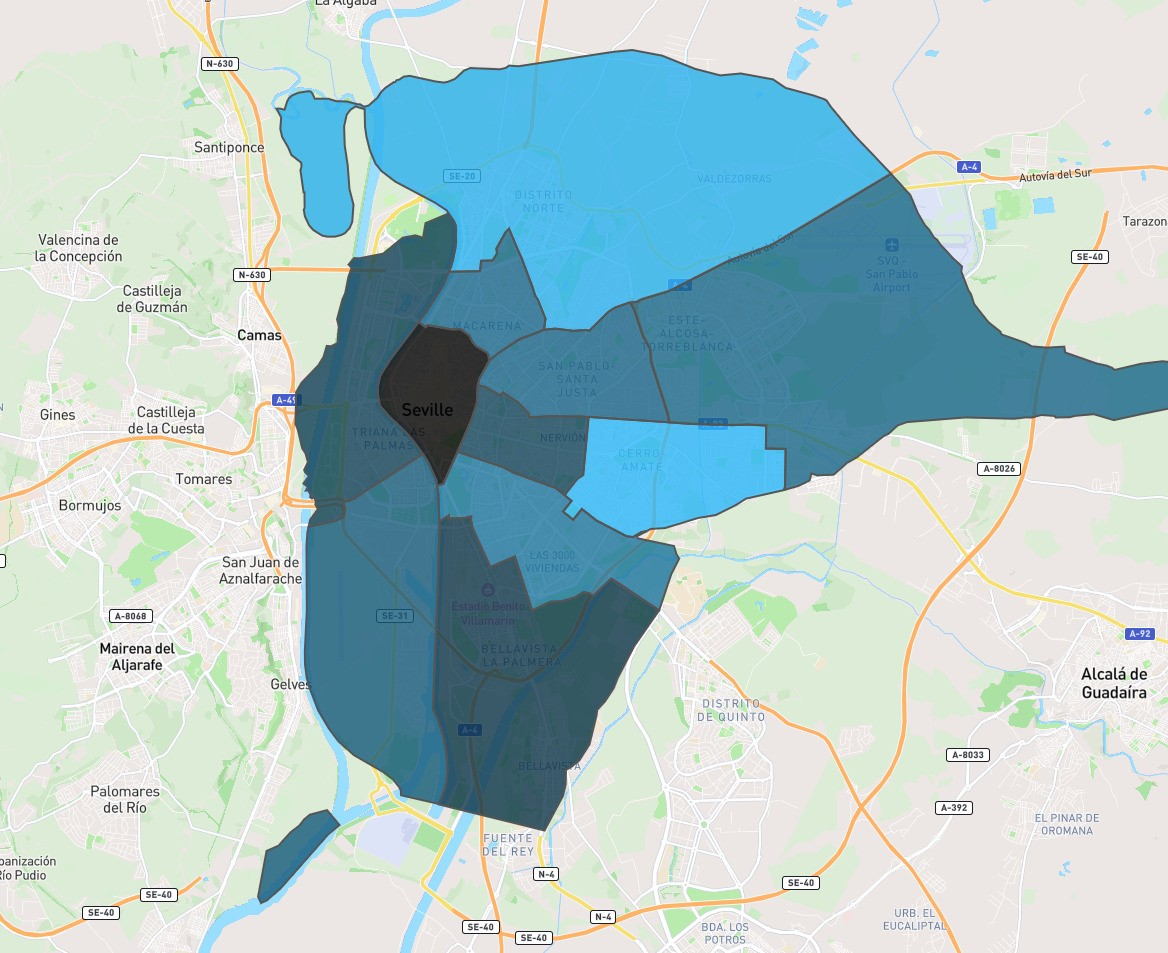
\includegraphics[width = 8.5cm, height = 8.08cm]{graphics/sevilledensity_map.jpeg}
                    \begin{flushleft}
                        \footnotesize{Fuente: elaboración propia a partir de \cite[(1)]{insideairbnb}}
                    \end{flushleft}
                \end{subfigure}
                \begin{subfigure}{0.5\textwidth}
                    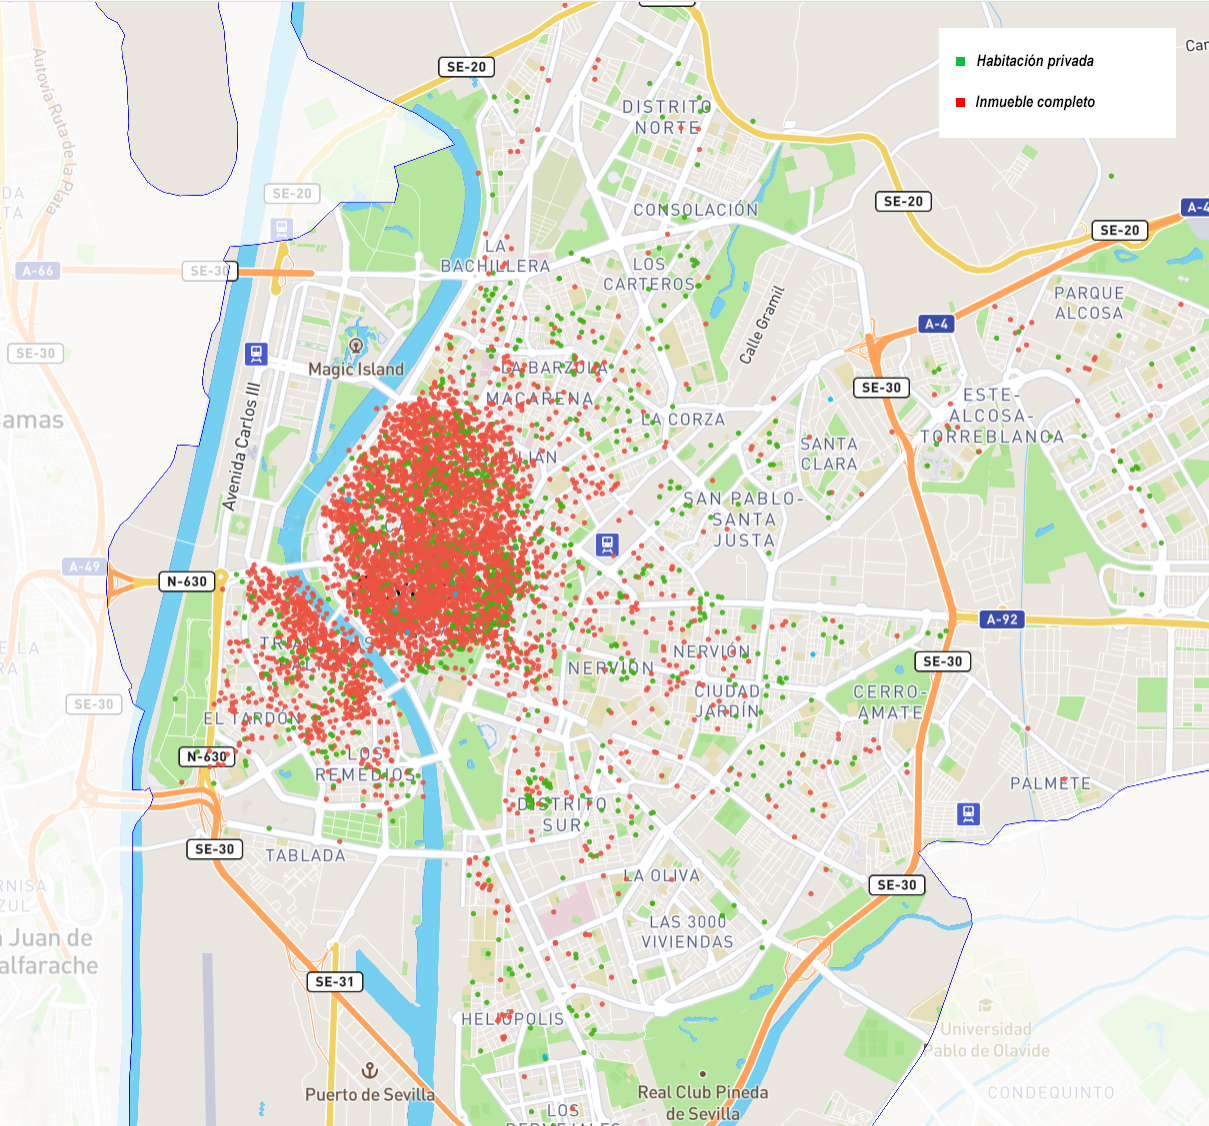
\includegraphics[scale = 0.4]{graphics/cap_sevilledensity_distribution_map.jpg}
                    \begin{flushleft}
                        \footnotesize{Fuente: \ \cite[(3)]{insideairbnb}}\\
                    \end{flushleft}
                \end{subfigure}
                \caption{Densidad por distritos y distribución de anuncios de alquiler turístico en la ciudad de Sevilla}
                
                \hfill \\
                En estas últimas imágenes se ve: a la izquierda, la densidad de la oferta según distritos sevillanos (a mayor saturación, mayor
                porcentaje de oferta tiene esa zona respecto al total); a la derecha, la distribución de anuncios de \airbnb \ del año 2022
                de la ciudad de Sevilla (en rojo, anuncios de inmuebles completos; en verde, anuncios de habitaciones privadas).

            \end{figure}

            Se ha oservado además la naturaleza de cada anunciante en los tres conjuntos de datos. Entiéndase como anunciante particular 
            aquel que posee 1 o 2 anuncios de inmuebles distintos en activo y como anunciante no particular u organización al que posee 3 o mas 
            anuncios. Entonces, los datos de Sevilla en 2018 nos reflejan que las organizaciones ostentaban un 38.7\% del mercado del alquiler turístico de 
            la ciudad, los de Sevilla en 2022 nos muestran un 53.25\% y los de España en 2018 un 39.46\%. Se ha observado pues que no solo ha aumentado
            el porcentaje del mercado controlado por organizaciones en Sevilla, sino que incluso en España las organizaciones que tienen un negocio
            alrededor del alquiler turístico controlan un gran sector del total. \\ 

            Finalmente, resulta interesante estudiar la variación de la actividad publicitaria de alquiler turístico en Sevilla tras el COVID.
            Los datos de 2018 y 2022 nos muestran una clara disminución de la actividad publicitaria. Mientras que en 2018 se recogieron 
            7424 anuncios de inmuebles en alquiler turístico en la ciudad de Sevilla, en 2022 se redujo la cifra a 6576. Además, 
            antes de la pandemia COVID, eran 3909 anunciantes o \textit{hosts} los que abarcaban la oferta en Sevilla, frente a los 2717 que
            se registraron en 2022. Es decir, ha disminuido el número de anunciantes. En términos porcentuales, los anuncios han disminuido 
            en un 11\% y los anunciantes en un 30\%.

        \clearpage

        \subsection{Resultados relativos al precio del alquiler turístico}
            
            \begin{figure}[ht]
                \begin{flushleft}
                    \includegraphics*[width = 15cm]{graphics/spain_2018_price.png}
                    \begin{flushright}
                        \footnotesize{Fuente: elaboración propia a partir de \cite[(1)]{datahippo} }
                    \end{flushright}
                    \caption{Precio por pernoctación en alquiler turístico en España, según comunidades autónomas}
                \end{flushleft}
            \end{figure}

            Como primer resultado de esta sección, se presenta un gráfico mostrando diferentes datos sobre el precio del alquiler turístico por noche en España, desagregado por comunidades autónomas, del año 2018. Antes de nada y para facilitar la compresión al lector, se explicará de forma escueta la interpretación de un gráfico como el que se muestra en pantalla: \textit{boxplot} o \textit{diagrama de cajas y bigotes}. Este tipo de gráfico muestra:
            una caja que representa el recorrido intercuartílico de la distribución, una línea divisoria en la caja que señala la mediana y unas vallas o \textit{bigotes} que delimitan los valores adyacentes a la mediana. En caso de que los hubiera, también se representan los datos anómalos o \textit{outliers}. En este caso, se han suprimido los \textit{outliers} por la gran cantidad de datos de la distribución. A su vez, no se entrará en detalles sobre qué delimita que un valor sea considerado adyacente o no a la mediana. Por último nótese que se ha marcado la media de la distribución completa.\\

            \noindent
            Entrando en materia podemos resaltar que las Islas Baleares es la comunidad con mayor mediana y cuyo rango intercuartílico se encuentra a un mayor precio, esto es el 50\% de los datos centrados en la mediana. Obsérvese que además la mediana se encuentra por delante de la media y es ligeramente superior a 100. Es decir, el 50\% de los anuncios de alquiler turístico de las Islas Baleares tienen un precio superior a 100€. Por otro lado, véase que las ciudades autónomas Ceuta y Melilla así como las Islas Canarias, Murcia, La Rioja e incluso la Comunidad de Madrid situán la mayoría de sus anuncios por debajo de la media nacional. 
                
            \clearpage

            \noindent
            Debe tenerse en cuenta la densidad de los datos, pues, por ejemplo, la Comunidad de Madrid cuenta con un gran número de anuncios de alquiler, tanto de alto como de bajo precio, lo que hace que su distribución se vea afectada, mientras que comunidades como Navarra que cuentan con muy pocos anuncios (véase [***]) pueden tener una distribución con precios más elevados debido a la presencia de tan solo un reducido número de datos con valores altos.
            Hablando de Andalucía, puede verse que la mayoría de sus datos se encuentran por debajo de la media nacional pero que también tiene un buen
            número de anuncios que sobrepasan este límite. 
            Por último destacan Navarra, el País Vasco, Cataluña y sobre todo las Islas Baleares como las comunidades que tienen anuncios con precios más elevados. En el caso de Baleares, existen datos, es decir, anuncios, que sobrepasan los 300€ por noche, y esto sin considerar los \textit{outliers}. \\

            \begin{figure}[ht]
                \begin{flushleft}
                    \includegraphics*[width = 13cm]{graphics/seville_2018_price.png}
                    \begin{flushright}
                        \footnotesize{Fuente: elaboración propia a partir de \cite[(2)]{datahippo} }
                    \end{flushright}
                    \caption{Precio por pernoctación en alquiler turístico en la ciudad de Sevilla, según distritos}
                \end{flushleft}

                Véase ahora este otro gráfico, del mismo estilo pero con datos relativos a la ciudad de Sevilla del año 2018.
                Primero de todo se ve que la mayoría de datos se encuentran por debajo de la media. Esto podría indicar la presencia 
                de un pequeño conjunto de datos con altos precios que afectan a la media de la distribución general.
                Exceptuando el Casco Antiguo, Nervión, Triana y el distrito Sur, el resto de distritos tienen su rango intercuartílico de 
                anuncios prácticamente por debajo de la media general. Este es un dato que muestra lo dispar que pueden ser los precios
                en la ciudad de Sevilla según los distritos. También, como en el anterior caso, se debe tener en cuenta la densidad de anuncios
                de cada zona (véase [***]). Por otro lugar, sin dudas el Casco Antiguo es el distrito líder en precios. Aun siendo el distrito con 
                mayor densidad, también es el que presenta no solo un mayor conjunto de datos con elevado precio sino además el máximo rango de precios de 
                ciudad. Sus \textit{bigotes} informan de anuncios en el distrito desde precios muy bajos hasta los más altos de la ciudad. 
                A esta zona le sigue Nervión, que aun tiendo bastantes anuncios por encima de la media, sitúa su mediana en un precio bastante económico.
                Por último, nótese que el distrito de La Palmera y Bellavista tiene casi la totalidad de sus datos por debajo de la media general. 
                Esto informa que mientras que sería complicado encontrar un inmueble de alquiler turístico en el Casco Antiguo por debajo de la media, 
                sería de mucha mayor facilidad encontrarlo por Bellavista o La Palmera. 

            \end{figure}

            \clearpage

            \begin{figure}[ht]
                \begin{flushleft}
                    \includegraphics*[width = 15cm]{graphics/seville_comparison_price.png}
                    \begin{flushright}
                        \footnotesize{Fuente: elaboración propia a partir de \cite[(2)]{datahippo} y \cite[(1)]{insideairbnb}}
                    \end{flushright}
                    \caption{Comparación de los precios por pernoctación en la ciudad de Sevilla entre los años 2018 y 2022}
                \end{flushleft}

                Se presenta aquí uno de los gráficos y resultados más importantes de la investigación. Se trata de la comparación de los
                precios por noche en alquiler turístico de la ciudad de Sevilla entre los años 2018 y 2022, antes y después de la pandemia.
                A simple vista se ve un claro incremento en general y en particular en todos los distritos del precio del alquiler turístico.
                La media, como se puede apreciar, se sitúa bastante más alta despues de la pandemia que anteriormente. Además, todos los distritos
                posicionan en 2022 el conjunto del 50\% de sus anuncios entorno a la mediana en márgenes de precios mayores que en 2018.
                La mediana también, en todos los casos, está por encima. Ahora bien, no todos los distritos han experimentado el mismo cambio.
                Por ejemplo, los precios en el distrito del Cerro - Amate o en el distrito Norte a penas han cambiado, exceptuando la aparición 
                de anuncios con precios más elevados y situados fuera de los recorridos intercuartílicos. Sin embargo, otros distritos, la mayoría,
                como Nervión, el Casco Antiguo, Los Remedios o Triana han pasado a tener un conjunto de anuncios con precios bastante mayores. De hecho, 
                la mediana de 2022 de muchos de ellos se sitúa por encima de todo el recorrido intercuartílico del año 2018.
                No obstante, se ha eludido hasta ahora el distrito de La Palmera y Bellavista. Esta zona ha experimentado el cambio más notable de todos, 
                superando no solo sus precios respecto a 2018 sino posicionándose como el distrito más caro en cuanto a alquiler turístico. Ha pasado de 
                ser un distrito con la mayoría de sus datos por debajo de la media a ser el que tiene mayor rango de precios, llegando a tener
                anuncios de 400€. Obsérvese que su tercer cuartil es también el mayor respecto al resto. Sin embargo muestra un rango 
                intercuartílico muy amplio y una mediana situada cerca de la media general, reflejando la gran diversidad de precios que presenta
                la zona.

            \end{figure}

            \clearpage
            
            \begin{wrapfigure}{l}{0.5\textwidth}
                \begin{flushleft}
                    \includegraphics*[width = 6cm]{graphics/seville_global_comparison_price.png}
                    \begin{flushleft}
                        \footnotesize{Fuente: elaboración propia a partir de \cite[(2)]{datahippo} y \cite[(1)]{insideairbnb}}
                    \end{flushleft}
                    \caption{Comparación global de los precios por pernoctación en la ciudad de Sevilla entre los años 2018 y 2022}
                \end{flushleft}
            \end{wrapfigure}

            \paragraph*{}
            Por último, se ha de fijar la atención en la variación global de los precios del alquiler turístico en la ciudad de Sevilla 
            entre los años 2018 y 2022. Lo más llamativo es que la media de 2022 se sitúa por encima de todo el recorrido intercuartílico de 
            la distribución de 2018. Esto apunta a que la gran mayoría de anuncios del año 2018 sitúan su precio por debajo de la media de 2022. 
            Pero es que, además, la media de 2018 se sitúa por debajo del 75\% de los datos de 2022, es decir, de los precios de los anuncios de este año.
            Esto nos da una idea de la enorme variación de precios en alquiler turístico que ha sufrido la ciudad de Sevilla. Nótese además
            la aparación de anuncios con precios mucho mayores a todos los existentes en 2018.

            \begin{wrapfigure}{R}{0.5\textwidth}
                \begin{flushright}
                    \includegraphics*[width = 9cm]{graphics/pricerelativevariation.png}
                    \begin{flushright}
                        \footnotesize{Fuente: elaboración propia a partir de \cite[(2)]{datahippo} y \cite[(1)]{insideairbnb}}
                    \end{flushright}
                    \caption{Distribución de densidad de la variación relativa del precio del alquiler turístico entre 2018 y 2022 en la ciudad de Sevilla}
                \end{flushright}
            \end{wrapfigure}

            \paragraph*{}
            A pesar de estos resultados, la investigación queda instatisfecha sobre el estudio de la variación del precio en el sector. Se 
            puede ir más allá.
            Para un análisis más valioso sobre la variación de los precios del alquiler turístico en la ciudad de Sevilla, se han tomado de 
            de los conjuntos de datos de 2018 y 2022 solo los anuncios coincidentes. Es decir, se han seleccionado los anuncios que estaban tanto
            en 2018 como en 2022. Los mismos inmuebles, ofrecidos por el mismo anunciante, pero en años diferentes. El estudio de la variación
            del precio sobre este subconjunto de datos es mucho más valioso al considererar exactamente el mismo servicio, pues son los mismos
            inmuebles los que se ofertan.

            \paragraph*{}
            \ \\

            Para obtener los resultados, previamente se han seleccionado las coincidencias, se han descartado 
            anuncios aparentemente anómalos y se han truncado los datos para un análisis más riguroso. Posteriormente se ha calculado la variación
            relativa del precio por noche de cada inmueble en 2022 respecto a su mismo anuncio en 2018. Los resultado pueden verse 
            en la Figura 8. La gráfica nos da mucha información, como que las variaciones relativas máximas se acercan a 1.5 y las mínimas 
            a -0.5 o que la mayoría de los anuncios han variado sus precios algo más del 0.1. Para simplificar, se ha marcado en rojo la media de 
            la distribución: 0.2375. Es decir, la variación media de los precios del alquiler turístico entre los años 2018 y 2022 en la ciudad de Sevilla
            es de 0.2375, o 23.75\%. Esto quiere decir que el precio ha aumentado en estos inmuebles un 23.75\%, una cifra considerablemente alta.
            Si comparamos esta variación con otros indicadores como el IPC o el IPV (Índice de Precios de la Vivienda), se ve lo alta que es la subida de 
            precios en este sector. Entre 2018 y 2022 el IPC varió un 12.16\% y el IPV un 19.46\% (véase \cite[(1) y (2)]{ine}), ambos por
            debajo de la variación de precios del alquiler turístico en Sevilla.

        \clearpage 

        \subsection{Resultados relativos a los inmuebles ofertados en alquiler turístico}

            \begin{figure}[ht]
                \begin{center}
                    \includegraphics*[width = 16cm]{graphics/tipoinmueble.png}
                    \begin{flushright}
                        \footnotesize{Fuente: elaboración propia a partir de \cite[(1) y (2)]{datahippo} y \cite[(1)]{insideairbnb}}
                    \end{flushright}
                    \caption{Tipos de inmuebles ofertados en alquiler turístico en la ciudad de Sevilla y España}
                \end{center}

                En este gráfico vemos los distintos inmuebles que los anunciantes ofrecen para el alquiler turístico. Por inmueble
                completo se entiende aquel que es un hogar en sí mismo y en el que el inquilino tiene total privacidad. Habitación privada
                corresponde al inmueble que ofrece una habitación propia para el inquilino y puede también incluir zonas 
                comunes a otros inquilinos. Por lo general una habitación privada no incluye todo lo necesario de un hogar. Y por habitación 
                compartida se entiende el mismo concepto que por habitación privada solo que ésta se comparte directamente con otros inquilinos. 
                Mirando los gráficos, vemos que tanto en España como en Sevilla predomina el inmueble completo aun teniendo un gran porcentaje 
                la habitación privada. Un resultado interesante es que la oferta de inmuebles completos en Sevilla ha ido en aumento desde 2018 
                y hasta 2022, teniendo en ese año un porcentaje del 85.5.

            \end{figure}

            \clearpage

    \setlength{\columnsep}{0.88cm}
    \begin{multicols}{2}

    \section{Conclusiones}

        \paragraph*{}
        Los resultados obtenidos informan sobre un sector escasamente estudiado. A pesar de la dificultad que entrañaba la investigación, se han podido
        clarificar y exponer datos que permiten conocer parte del alquiler turístico a nivel nacional y en la ciudad de Sevilla. Además, se han
        conseguido presentar resultados de manera desagregada, hecho singular. 
        
        \paragraph*{}
        Por un lado se ha estudiado la distribución de la oferta del alquiler 
        turístico, donde se ha constatado que Andalucía y Cataluña en España y el Casco Antiguo en Sevilla son los territorios con mayor porcentaje
        de anuncios. Además se ha estudiado como ha variado esta distribución tras la pandemia en Sevilla y se ha visto el aumento del predominio del 
        Casco Antiuo como principal zona ofertante. Asimismo, se ha visto qu elas provincias de Barcelona y Madrid destacan como líderes en oferta de alquiler turístico. Posteriormente, se han analizado los precios de los anuncios por distritos en la ciudad de Sevilla y por comunidades autónomas en España.
        Las Islas Baleares han resultado la comunidad autónoma con mayores precio de alquiler turístico, al igual que el Casco Antiguo en Sevilla, que 
        vuelve a destacar. Se llegó entonces a la parte más importante y valiosa de la investigación: la comparación de los precios del alquiler turístico
        de la ciudad de Sevilla entre los años 2018 y 2022. Se arrojaron entonces resultados sorprendentes, como el cambio de papel que experimentó el distrito 
        de la Palmera y Bellavista pasando de ser una zona rezagada a ser líder en precios. Además se confirmó la alta subida de precios que había sufrido la ciudad, tanto en general como en cada distrito. A su vez se estudió la variación de los precios después de la pandemia sobre un subconjunto de 
        inmuebles de los que se tenían datos tanto de 2018 como de 2022. Aquí se terminó de fundamentar la alta variación de precios que se había dado en el 
        sector, superando incluso las variaciones de índices como el IPC o el IPV. Por último se vieron los diferentes tipos de inmueble que se ofertaban
        en el sector y el predominio del inmueble completo. 

        \paragraph*{}
        En definitiva, se han cumplido y abordado todos los objetivos que fueron propuestos. Más aún, se ha ofrecido iformación adicional que ha 
        ido apareciendo a lo largo del proceso de investigación. 
        
        \paragraph*{}
        Por otra parte, el presente trabajo tiene la intención de abrir camino en un sector,
        como ya se ha dicho, poco estudiado. Este texto demuestra la posibilidad de estudiar el alquiler turístico de manera desagregada. De hecho es
        tan solo un acercamiento a todo el estudio que se podría llegar a hacer con más medios y tiempo que de los que disponía el autor. Pero incluso 
        de esta manera se han expuesto resultados interesantes y de gran ayuda para el estudio económico y estadístico de otros temas relacionados.
        Por ello se incentiva a otros investigadores a abrir nuevas vías de estudio sobre el alquiler turístico. Por ejemplo, se podría 
        plantear el estudio del alquiler turístico a nivel europeo de manera desagregada o el seguimiento de los datos del sector a nivel nacional durante 
        un periodo considerable de años. 

        \paragraph*{}
        Estas propuestas no son ilusorias, pues empresas de alquiler turístico como \airbnb \ u otras son fuentes de datos lo suficientemente grandes
        como para abarcar un proyecto de tal índole. Aunque con necesidad de trabajo, los datos están ahí, esperando a ser tratados para la obtención de 
        resultados que ayuden a entender mejor este sector y a la economía en general.

    \begin{thebibliography}{20}

            \bibitem[DataHippo]{datahippo} 
                \ 
                \begin{enumerate}
                    \item \href{https://datahippo.org/es/region/599216cb8a4655339b819813/}{Datos España 2017 - 2018}
                    \item \href{https://datahippo.org/es/region/599230af8a46554edf884651/}{Datos Sevilla 2017 - 2018}
                    \item \href{https://datahippo.org/media/regions/58612732-b2dc-433b-ab78-b8fbe5bbbb16/599216cb8a4655339b819813_airbnb.csv}{Datos España 2017 - 2018 (CSV)}
                    \item \href{https://datahippo.org/media/regions/7e3f7365-8ec0-42f1-a277-9b82743b8a39/599230af8a46554edf884651_airbnb.csv}{Datos Sevilla 2017 - 2018 (CSV)}
                \end{enumerate}
            
            \bibitem[InsideAirbnb]{insideairbnb}
                \
                \begin{enumerate}
                    \item \href{http://insideairbnb.com/get-the-data/}{Datos Sevilla 2022}
                    \item \href{http://data.insideairbnb.com/spain/andaluc%C3%ADa/sevilla/2023-03-31/visualisations/listings.csv}{Datos Sevilla 2022 (CSV)}
                    \item \href{http://insideairbnb.com/sevilla}{Distribución de anuncios de alquiler turístico en la ciudad de Sevilla (Figura 3.2)}
                \end{enumerate}

            \bibitem[INE]{ine}
                \
                \begin{enumerate}
                    \item \href{https://www.ine.es/jaxiT3/Datos.htm?t=50934}{Variación anual del IPC (2018 - 2022)}
                    \item \href{https://www.ine.es/jaxiT3/Datos.htm?t=25173}{Variación anual del IPV (2018 - 2022)}
                \end{enumerate}

    \end{thebibliography}
        
    \hypertarget{anexo}{}
    \section*{Anexo}

        \hypertarget{github}{[GitHub] \href{https://github.com/m7pantoja/TouristRental}{Repositorio de código sobre el proceso de investigación}}

    \end{multicols}
    \setlength{\columnsep}{10pt}

\end{document}




% Consideraciones: 
% - Me he descargado el pdf, y me salen algunos enlaces enmarcados en rojo, otros en verde y otros en azul. No se si es intencionado, no es que me disguste pero que sepas que se ve así 
% (imagino que dependerá de si son enlaces internos o externos)